\documentclass{article}
\usepackage{graphicx}
\usepackage[export]{adjustbox}
\usepackage[spanish]{babel}
\usepackage[utf8]{inputenc}
\usepackage{indentfirst}
\usepackage{float}
\usepackage{subfig}
\usepackage{booktabs}
\usepackage{pgfplots}
\usepackage{listings}
\usepackage{fancyhdr}
\setlength{\parskip}{1ex}
\usepackage{amssymb,amsmath}
\usepackage[hidelinks]{hyperref} 
\graphicspath{{C:/Users/Gustavo/Documents/Electrónica/7.- Semestre/Control/Reportes\P1}}
\usepackage[left=2.5cm,
			top=2.5cm,
			right=2.5cm,
			bottom=3cm]{geometry}
\lstset{language=Scilab, breaklines=true, basicstyle=\footnotesize}
\lstset{numbers=left, numberstyle=\tiny, stepnumber=2, numbersep=-8pt}

%Materia y maestro
\newcommand{\materia}{\uppercase{Control I}}
\newcommand{\maestro}{\uppercase{M.C. Gerardo Marx Chávez-Campos}}

%Tipo de documento y nombres de tema
\newcommand{\tipoDoc}{\uppercase{}} %TAREA, REPORTE DE LABORATORIO,
\newcommand{\nombreDoc}{\uppercase{Reporte Práctica No. 1}} 
\newcommand{\docNum}{}
\newcommand{\subNombreDoc}{\uppercase{Analysis of a first order system}}

%Alumnos y fecha
\newcommand{\alumnos}{Gustavo Martínez Mondragón \\
	Carlos Alberto Del Portillo Malandra}
\newcommand{\fecha}{\uppercase{26 de octubre de 2017}}



\begin{document}
	%Cabezal del membrete
	\begin{center}
		
\includegraphics[scale=.5]{encabezado}
		\vspace{.3cm}
		\hrule height2.5pt
		\vspace{.1cm}
		\hrule height1pt
		\vspace{.3cm}
		\huge INSTITUTO TECNOLÓGICO DE MORELIA \\
		\vfill
		\large DIVISIÓN DE ESTUDIOS PROFESIONALES  \\
		\vfill
		\large  DEPARTAMENTO DE INGENIERÍA ELECTRÓNICA \\ 
		\vfill
		\Large \textbf \materia \\
		\vfill
		\textbf{\tipoDoc} \\
		\vfill 
		\LARGE  \textbf{ \nombreDoc  \, \docNum: \\ \subNombreDoc} \\
		\vfill
		\large PRESENTA(N): \\
		\large  \textbf{\alumnos} \\
		\vfill
		\large PROFESOR: \\
		\Large \textbf{\maestro }
		\vfill 
	\end{center}
	\begin{flushleft}
		MORELIA, MICHOACÁN \hfill \uppercase{\fecha}
	\end{flushleft}
	
	
	
	\thispagestyle{empty} 
	\newpage
	\tableofcontents
	\thispagestyle{empty}
	\newpage
	\pagestyle{fancy}
	\lhead{Control I}
	\chead{Práctica No. 1}
	\rhead{\alumnos}
	\section{Introducción}
	
	Se formulará la representación de un sistema hidráulico a través de una función algebraica, la cual relaciona la salida con la entrada,a esta expresión se le conoce como \textbf{función de transferencia}; esta tiene dos formas de ser expresada: En el dominio de la frecuencia la cual se obtiene utilizando la \textbf{transformada de Laplace}. También se encontrará la respuesta en el dominio del tiempo del sistema hidráulico \textbf{utilizando la transformada inversa de Laplace}.
	
	Posteriormente, se implementará la respuesta en el dominio del tiempo en una función de Scilab, y con ayuda de este código, se encontrara la gráfica para los siguientes casos:
\begin{enumerate}
	\item $ \omega_i(t)>\omega_o(t) $
	\item $ \omega_i(t)<\omega_o(t) $
	\item  $ \omega_i(t)=\omega_o(t) $
\end{enumerate}

	Por último se compararán los resultados obtenidos con la función de Scilab.

	\section{Metodología}
	\subsection{Desarrollo teórico}
	
	Se tiene el siguiente sistema hidráulico de entrada $ W_i(t) $ y salida $W_o(t) $ en la Figura \ref{hidr}.
	
	\begin{figure}[H]
		\centering
		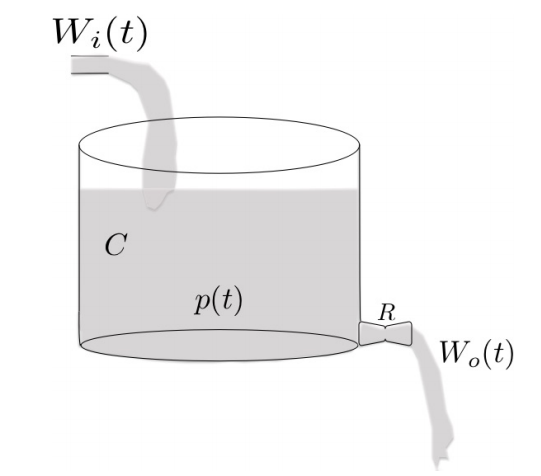
\includegraphics[width=0.55\linewidth]{hidr}
		\caption{Esquema de sistema hidráulico.}
		\label{hidr}
	\end{figure}
	
	
	Se obtuvo la ecuación diferencial que define el comportamiento de dicho sistema, que depende de la altura del agua del recipiente ($ h(t) $).	
	\begin{align}
	\omega_i(t)=A\frac{dh(t)}{d(t)}+R\frac{h(t)}{rg}
	\end{align}
	
	
	 Luego se propuso la analogía eléctrica de nuestro sistema hidráulico, en la cual optamos por usar un circuito de corriente como se muestra en la Figura \ref{circ}
	
	\begin{figure}[H]
		\centering
		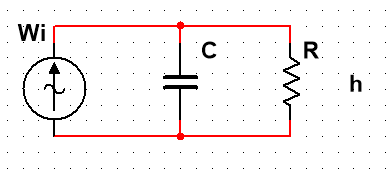
\includegraphics[width=0.7\linewidth]{circuito}
		\centering
		\caption{Analogía eléctrica del sistema hidráulico}
		\label{circ}
	\end{figure}
	  
	 Entonces la ecuación de nuestra analogía es:
	 
	 \begin{equation}
	 \begin{split}
 \omega_i(t)=C\frac{dh(t)}{dt}+\frac{h(t)}{R}\\
donde:\quad R=\frac{R}{rg}\quad y\quad C=A
	 \end{split} \label{ana}
	 \end{equation}
	 
	 Usando transformada de Laplace y factorizando H(s).
	 \begin{align}
	 \omega_i(t)= CsH(s)+ \frac{H(s)}{R}\\ \label{eqs}
	 \omega_i(s)=H(s)\left[Cs+\frac{1}{R}\right]
	 \end{align}
	 Despejando H(s) y pasar dividiendo al factor que multiplicaba a H(s) y factorizando se obtiene la función de transferencia 
	 \begin{align}
	 \frac{H(s)}{\omega_i(s)}=\frac{1}{Cs+ \frac{1}{R}}\\
\frac{H(s)}{\omega_i(s)}=\frac{1}{C}\left(\frac{1}{s+\frac{1}{RC}}\right)\\
\frac{H(s)}{\omega_i(s)}=\frac{\frac{1}{C}}{S+\frac{1}{RC}}
	 \end{align} 
	 
	 La función de transferencia de un sistema de primer orden se puede expresar también de la forma general.
	 \begin{equation}
	 \begin{split}
	 G(s)=\frac{bs+c}{ds+a}\\
	 donde:\quad a=\frac{1}{RC},\quad b=0,\quad c=\frac{1}{C}\quad y \quad d=1
	 \end{split} \label{trans}
	 \end{equation}
	 Sabemos que la respuesta al impulso del sistema se describe de la siguiente manera
	 \begin{equation}
	 Y(s)=\frac{1}{s}\left(\frac{bs+c}{ds+a}\right)
	 \end{equation}
	 Para encontrar la respuesta del sistema al impulso en el dominio del tiempo se debe escribir en forma de fracciones parciales y obtener la transformada inversa de Laplace
	 \begin{align}
	 \frac{bs+c}{s(ds+a)}=\frac{A}{s}+\frac{B}{ds+a}\\
	 obtenemos:\quad A=\frac{c}{a}\quad y\quad B=b-\frac{dc}{a}\\
	 Y(s)=\frac{\frac{c}{a}}{s}+\frac{b-\frac{dc}{a}}{ds+a}\\
	 Y(s)=\frac{\frac{c}{a}}{s}+\frac{b-\frac{dc}{a}}{d(s+\frac{a}{d})}\\
	 Y(s)=\frac{c}{a}\frac{1}{s}+\frac{b-\frac{dc}{a}}{d}\frac{1}{s+\frac{a}{d}}\\
	 y(t)= \frac{c}{a}u_s(t)+\left(\frac{b}{d}-\frac{c}{a}\right)e^{\frac{-a}{d}t}u_s(t) \label{rt}
	 \end{align} 
	 
	 \subsection{Código}
	 En el código de nuestra función para representar gráficamente la respuesta del sistema en el dominio del tiempo, se utilizó \eqref{rt}, con un vector t, se realiza un barrido en el tiempo a la respuesta en el tiempo, y posteriormente se grafica como se ve en el Listado 1.
	 \lstset{language=Scilab}
	 \begin{lstlisting}[frame=single]
function[y]=STF(a,b,c,d) //Se establece la salida y y los parametros de entrada a,b,c y d
t=0:0.02:10; //Se establece un vector de tiempo de 0 a 10 con incrementos de 0.02
y=(c/a)+((b/d)-(c/a))*exp((-a/d)*t); //Respuesta del sistema al impulso en el tiempo
plot(t,y) //Se grafica la respuesta del sistema y contra el tiempo t
endfunction 
	 \end{lstlisting} 
	 
	 Para obtener los 3 casos que se mencionaron con anterioridad, se realizaron los siguientes cálculos:

	 Para$\quad \omega_i(t)>\omega_o(t)$, se usa la ecuación \eqref{eqs} y se toma $ \omega_i(t) $ como entrada y $ \frac{h(t)}{R} $ como salida, entonces, se propone un valor de 2 para la entrada y uno menor de 1 para la salida, quedando la ecuación de la siguiente manera:
	 
	 \begin{align}
	\omega_i(t)= CsH(s)+ \frac{H(s)}{R}\\
	2= x+1\\
	x=2-1=1
	 \end{align}
	 
	 Entonces en \eqref{trans}, a sería el valor de la salida (a=1), el valor del capacitor C lo tomaría d=1, como no hay s alguna en el numerador, b=0 y c es el numerador con valor de 1.
	 
	  Para$\quad \omega_i(t)<\omega_o(t)$, se propone un valor de 1 para la entrada y uno mayor de 2 para la salida, quedando la ecuación de la siguiente manera:
	 
	 \begin{align}
	 1= x+2\\
	 x=1-2=-1
	 \end{align}
	 
	 Entonces en \eqref{trans}, a sería el valor de la salida (a=2), el valor del capacitor C lo tomaría d=-1, como no hay s alguna en el numerador, b=0 y c es el numerador con valor de 1.
	 
	  Para$\quad \omega_i(t)=\omega_o(t)$, se da un valor de 1 a todos los coeficientes, ya que de esta manera se evita la indeterminación en \eqref{rt}.
	  
	  \section{Resultados y Observaciones}
	  
	  A continuación se muestra la respuesta al impulso del sistema para los tres caso solicitados usando la función desarrollada por código.
	  
	  \begin{figure}[H]
	  	\centering
	  		  	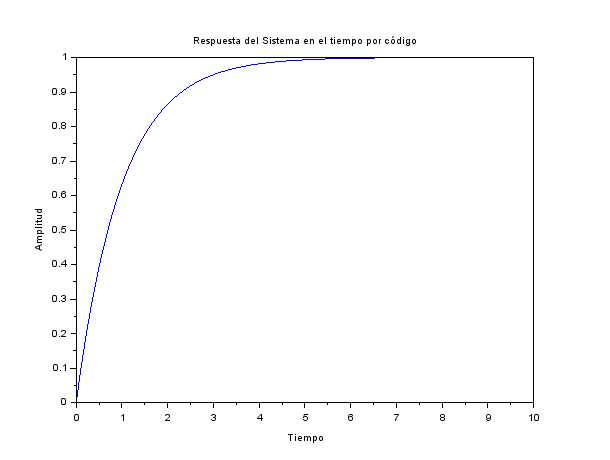
\includegraphics[scale=0.55]{mayor.PNG}
	  	\centering
	  	\caption{Respuesta al impulso del sistema cuando $ \omega_i > \omega_o $ con función por código}
	  \end{figure}
	  
	  
	    \begin{figure}[H]
	  	\centering
	  	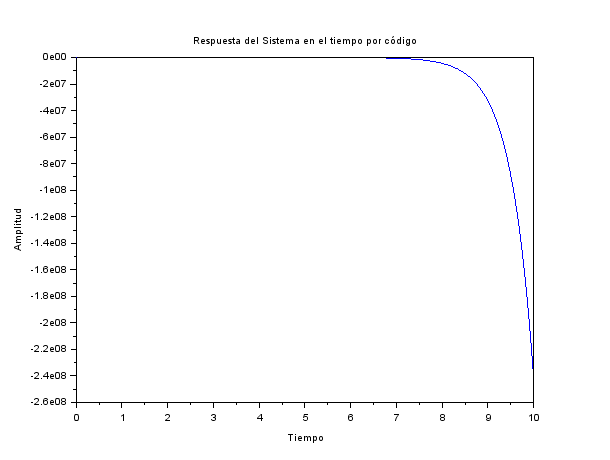
\includegraphics[scale=0.55]{menor.PNG}
	  	\centering
	  	\caption{Respuesta al impulso del sistema cuando $ \omega_i < \omega_o $ con función por código}
	  \end{figure}
	  
	    \begin{figure}[H]
	  	\centering
	  	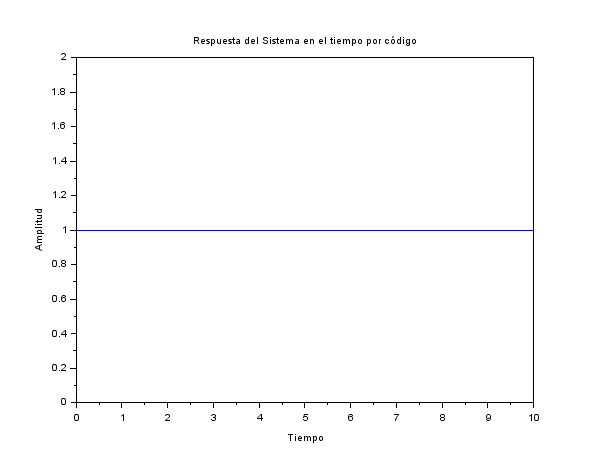
\includegraphics[scale=0.55]{igual.PNG}
	  	\centering
	  	\caption{Respuesta al impulso del sistema cuando $ \omega_i = \omega_o $ con función por código}
	  \end{figure}
	
	Se muestra el código usado para emplear la función de transferencia por medio de Scliab en el Listado 2.
	\begin{lstlisting}[frame=single]
	s=%s 
	K=1;
	Tau=1;
	simpleSys=syslin('c',K/(1+Tau*s))
	t=0:0.02:20;
	y=csim('step',t, simpleSys)
	plot(t,y)
	xtitle("Respuesta del Sistema en el tiempo por Scilab", "Tiempo", "Amplitud")
	\end{lstlisting}
	
	A continuación se muestran las gráficas de la respuesta al impulso del sistema usando las funciones de Scilab, solo se tiene que considerar que Tau=d, K=c y el 1 que se suma con el factor Tau*s irá tomando los valores de a. Cabe destacar que se obtienen los mismos resultados que con la función desarrollada por medio de código.
	
	
	\begin{figure}[H]
		\centering
		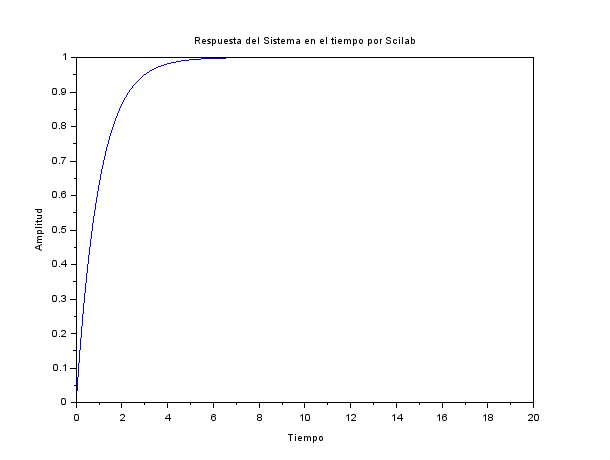
\includegraphics[scale=0.55]{mayor1.PNG}
		\centering
		\caption{Respuesta al impulso del sistema cuando $ \omega_i > \omega_o $ con función por Scilab}
	\end{figure}
	
	
	\begin{figure}[H]
		\centering
		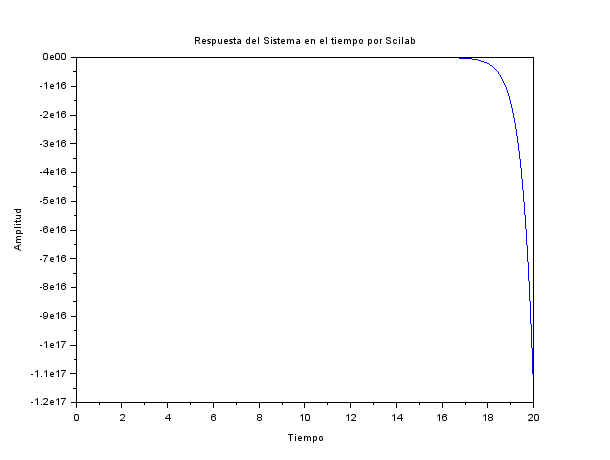
\includegraphics[scale=0.55]{menor1.PNG}
		\centering
		\caption{Respuesta al impulso del sistema cuando $ \omega_i < \omega_o $ con función por Scilab}
	\end{figure}
	
	\begin{figure}[H]
		\centering
		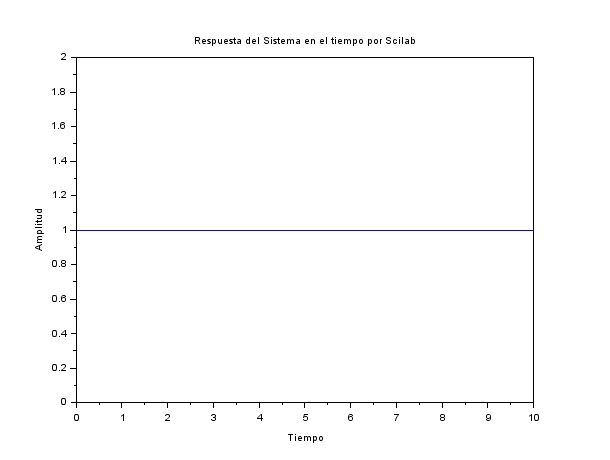
\includegraphics[scale=0.5]{igual1.PNG}
		\centering
		\caption{Respuesta al impulso del sistema cuando $ \omega_i = \omega_o $ con función por Scilab}
	\end{figure}

\subsection{Observaciones}
\textbf{Carlos Alberto Del Portillo Malandra:} Al simular el código en Scilab pudimos observar el comportamiento de un sistema hidráulico. En el caso en el que la entrada es mayor a la salida observando el comportamiento de un capacitor cuando éste se está carga, posteriormente, se observó el caso cuando la salida es mayor a la entrada observando en éste la analogía de descarga del capacitor y en el último se puede observar como la respuesta es constante al ser iguales la salida y la entrada, dando gráficamente una linea recta.

\textbf{Gustavo Martínez Mondragón:} Lo que se puede observar en las gráficas de ambos códigos (el propio y el de Scilab) son resultados idénticos, también se puede observar que cuando la entrada supera a la salida, el sistema tenderá a llenarse, como el fenómeno de un capacitor al cargarse, de igual manera cuando se tiene una salida mayor que la entrada se puede ver una descarga, mientras que al ser iguales ambos el flujo permanecerá constante.

\section{Conclusiones}
\textbf{Carlos Alberto Del Portillo Malandra:} En la realización de esta práctica se pudo reforzar el conocimiento de circuitos RC de cursos anteriores con la interpretacion de un sistema hidráulico haciendo analogía a un sistema eléctrico desarrollando con la ayuda de la transformada y transformada inversa en de Laplace obteniendo como resultado la función de trasferencia del sistema. 

\textbf{Gustavo Martínez Mondragón:} Lo que podemos concluir al realizar nuestro código para obtener la respuesta de un sistema de primer orden como lo fue el sistema hidráulico es que cualquier sistema simple tendrá una respuesta en el dominio del tiempo regido por \eqref{rt} que es dependiente de sus coeficientes; por lo que se puede decir que el algoritmo que usa Scilab usa la misma ecuación a la que llegamos nosotros. También como ya se ha visto en clase, para nosotros los ingenieros en electrónica resulta más sencillo analizar sistemas ajenos a nuestro campo de aplicación al hacer analogías, ya que la gran mayoría se rige por ecuaciones diferenciales, por lo que dominar herramientas como la transformada de Laplace y su inversa es de gran importancia.

	
	
\end{document}